%\documentclass[journal]{IEEEtran}
%\documentclass[12pt,onecolumn]{IEEEtran}
\documentclass[UTF8]{article}
\usepackage{ctex}
\usepackage{geometry,graphicx,marvosym}
\usepackage{amsmath,amsthm}
\usepackage{amsfonts}
\usepackage[usenames,dvipsnames]{pstricks}
\usepackage{pst-plot,pstricks-add}
%\usepackage{graphicx,times,amsmath,amssymb,multirow,subfigure}
\usepackage{graphicx,times,amsmath,amssymb,multirow}
\usepackage{url}
\usepackage{stfloats}
\usepackage{amsfonts,rotating}
\usepackage{color}
\usepackage{verbatim,multirow}
% setting dimension of the paper
\textwidth 7.0true in
\textheight 8.9 true in
\topmargin=-20pt
\headheight=6pt
\headsep=2pt
\oddsidemargin -0.3true in
\evensidemargin -0.4true in
\usepackage{amssymb}

\newtheorem{theorem}{Theorem}
\newtheorem{lemma}{Lemma}
\newtheorem{algorithm}{Algorithm}
\newtheorem{definition}{Definition}
\newtheorem{proposition}{Proposition}

\newcommand{\dtcwt}{\operatorname{DT-\mathbb{C}WT}}
\newcommand{\tpctf}{\operatorname{TP-\mathbb{C}TF}}
\newcommand{\ctf}{\operatorname{\mathbb{C}TF}}
\newcommand{\tr}[1]{\textcolor{red}{#1}}
\newcommand{\tb}[1]{\textcolor{blue}{#1}}
\newcommand{\mO}{{\mathcal{T}}}
\newcommand{\C}{\mathbb{C}}    %complex number field
\newcommand{\N}{\mathbb{N}}    %natural numbers
\newcommand{\R}{\mathbb{R}}    %real number field
\newcommand{\Z}{\mathbb{Z}}    %integers
\newcommand{\imag}{\mathrm{i}} % imaginary unit
\newcommand{\dR}{\mathbb{R}^d}
\newcommand{\dT}{\mathbb{T}^d}
\newcommand{\dZ}{\mathbb{Z}^d}
\newcommand{\dlp}[1]{l_{#1}(\mathbb{Z}^d)}
\newcommand{\td}{\boldsymbol{\delta}}  %Dirac/Kronicker sequence
\newcommand{\bp}{\begin{proof}}
	\newcommand{\ep}{\hfill  \end{proof} }
\newcommand{\be}{ \begin{equation} }
	\newcommand{\ee}{ \end{equation} }
\newcommand{\dLp}[1]{L_{#1}(\mathbb{R}^d)}
\newcommand{\prm}{P}           %projection matrix
\newcommand{\wh}{\widehat}
\renewcommand{\le}{\leqslant}
\renewcommand{\ge}{\geqslant}
\newcommand{\bs}{\backslash}
\newcommand{\ol}{\overline}
\newcommand{\vk}{\mathsf{k}}
\newcommand{\la}{\langle}
\newcommand{\ra}{\rangle}
\newcommand{\tp}{\mathsf{T}}  %transpose
\newcommand{\conj}{\overline}
\newcommand{\supp}{\mathrm{supp}}
\newcommand{\setsp}{\;:\;}     %set separator
\newcommand{\sd}{\mathcal{S}}  %subdivision operator S
\newcommand{\tz}{\mathcal{T}}  %transition operator T
\newcommand{\wt}{\widetilde}
\renewcommand{\le}{\leqslant}
\renewcommand{\ge}{\geqslant}
\newcommand{\er}{\eqref}
\newcommand{\gep}{\varepsilon}
\newcommand{\eps}{\epsilon}
\newcommand{\gl}{\lambda}
\newcommand{\gL}{\Lambda}
\newcommand{\gd}{\delta}
\newcommand{\DAS}{\mathrm{DAS}}
\newcommand{\UDAS}{\mathrm{UDAS}}
\newcommand{\DHF}{\mathrm{DHF}}
\newcommand{\bm}{\boldmath}
\newtheorem{example}{Example}
\bibliographystyle{unsrt}
\newcommand{\xz}[1]{\textcolor{magenta}{\bf #1}}
\usepackage[colorlinks,linkcolor=blue,anchorcolor=blue,citecolor=blue]{hyperref}
\usepackage{indentfirst}
\usepackage{subcaption}

\usepackage{geometry}
\geometry{a4paper,scale=0.8}
\boldmath
\begin{document}
	\author{Huang Yijun}
\title{Report : Exploiting 3D Framlets to Extract Structrual Sparsity from 3D patches}
\maketitle

\section{基于Patch的重建模型}
\par 假设 $u\in R^N$ 是MRI图像的向量形式,则图像$u$可以被划分为若干个具有重叠位置且大小为$\sqrt{n} \times \sqrt{n}$的图像patch。若给定一个目标图像patch,我们可以通过在该MRI图像中寻找其相似patch,并将这些相似patch通过堆叠的方式组成3D patch结构,进而使用3D紧框架提取特征。因此,使用算子$R_i$表示图像块匹配操作,即$R_i x$表示通过图像块匹配操作将第$i$个patch与其相似patch构造成3D结构,则我们可以写出如下模型:
\begin{equation}
	min \quad \frac{1}{2}\Vert Mu - g \Vert_2^2 + \lambda \sum_i^I  \Vert WR_iu \Vert_1
\end{equation}
其中 $M = PFS$,$P$为采样矩阵,$F$为傅里叶变换, $S$是线圈灵敏度矩阵,$g$表示k空间欠采样数据, $W$是3D紧框架变换矩阵, $\lambda$为正则化参数,用于权衡数据精确项和稀疏项。
\par 如图1所示,该图说明了算子$R_i$具体的操作流程,首先对于目标patch,我们使用patch match的算法寻找对应目标patch的相似patch,然后将所有patch堆叠成三维的结构(需要按照相似性进行排序),然后对该三维结构的数据进行三维紧框架变换,得到三位紧框架系数,紧接着使用软阈值算法对系数去伪影或者噪声,对处理后的系数进行重构,最后将重构后的数据放回原图中,即$R_i^T$操作。

\begin{figure}[h]   
	\centering         %使图片居中放置
	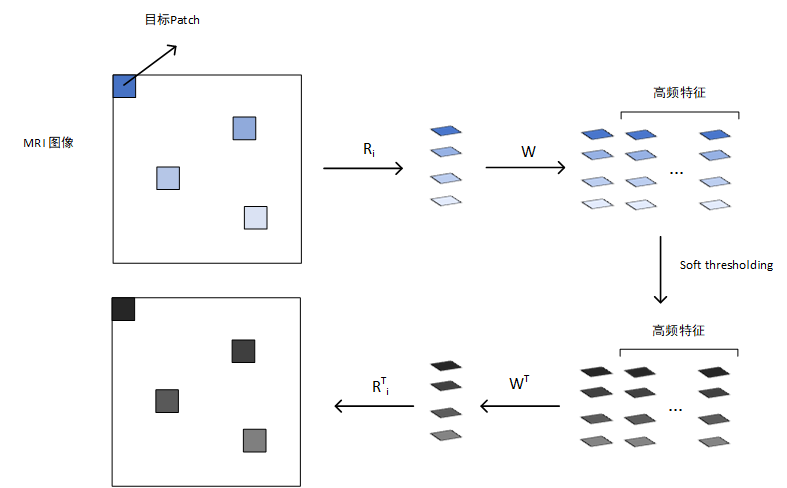
\includegraphics[scale=0.6]{patch.png}
	\caption{图像块匹配$R_i$,及其伴随算子$R_i^T$等说明。}
\end{figure}

\section{模型求解} 
\par 模型(1)是一个Group Lasso问题,因此可以直接通过ADMM求解,模型可以重新写为:
\begin{equation}
	\begin{aligned}
		min \quad& \frac{1}{2}\Vert Mu - g \Vert_2^2 + \lambda \sum_i^I  \Vert z_i \Vert_1 \\
		s.t. \quad& WR_iu = z_i, i= 1,\dots, I
	\end{aligned}
\end{equation}
模型(2)的增广拉格朗日形式为:
\begin{equation}
	min \quad \frac{1}{2}\Vert Mu - g \Vert_2^2 + \lambda \sum_i^I  \Vert z_i \Vert_1 + \frac{\rho}{2} \sum_i^I (\Vert WR_iu - z_i + y \Vert_2^2 - \Vert y\Vert_2^2)
\end{equation}
其中$y$是对偶变量,$\rho > 0$。则ADMM算法迭代如下:
\begin{equation}
	\begin{aligned}
		u^{k+1} & =  (M^TM+\rho \sum_i^I R_i^TR_i )^{-1} (M^Tg - \rho \sum_i^I R_i^T W^T (y^{k}-z_i^{k})) \\
		z_i^{k+1} &= soft( WR_iu^{k}  + y^{k}, \frac{\lambda}{\rho}) \\
		y^{k+1} & = y^{k} + WR_iu^{k} - z_i^{k}
	\end{aligned}
\end{equation}
其中$\sum_i^I R_i^TR_i$ 表示每个像素点被分配到patch相似组中的次数。
\end{document}